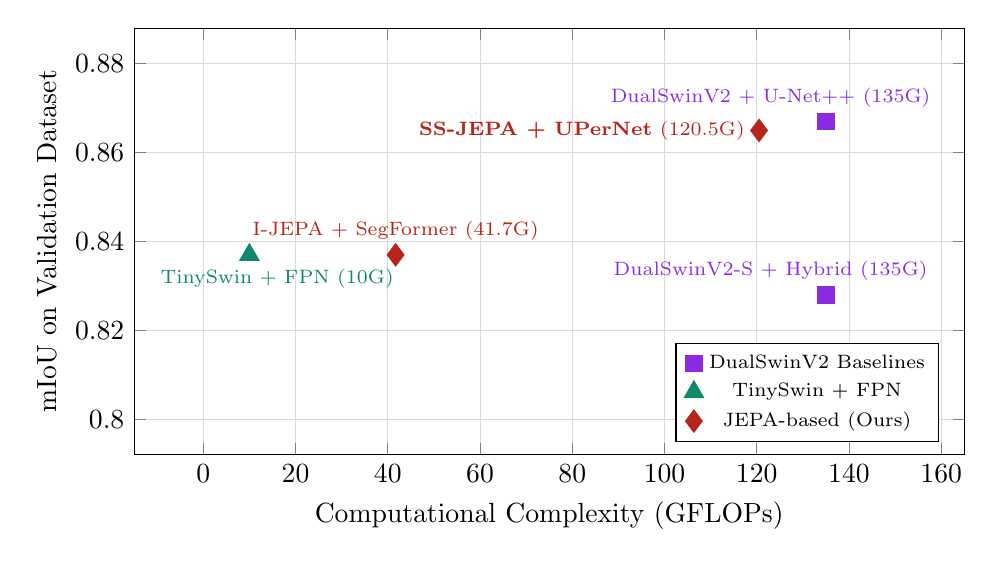
\begin{tikzpicture}
	\begin{axis}[
			width=\linewidth,
			height=7cm,
			xlabel={Computational Complexity (GFLOPs)},
			ylabel={mIoU on Validation Dataset},
			grid=both,
			grid style={line width=.1pt, draw=Gray!10},
			major grid style={line width=.2pt, draw=Gray!30},
			xmin=0, xmax=150,
			ymin=0.80, ymax=0.88,
			legend pos=south east,
			legend style={font=\scriptsize, fill, draw},
			enlarge x limits={rel=0.1},
			enlarge y limits={rel=0.1},
			title style={font=\bfseries},
			% Positioning labels automatically
			nodes near coords,
			point meta=explicit symbolic,
			every node near coord/.append style={
					font=\scriptsize,
					anchor=south,
					inner sep=5pt,
				}
		]

		% Data for Baselines (Standard Models)
		\addplot[
			only marks,
			mark=square*,
			mark size=3pt,
			BlueViolet,
			every node near coord/.append style={xshift=-20pt}
		] table [meta=label] {
				x   y   label
				135.0 0.867 {DualSwinV2 + U-Net++ (135G)}
				135.0 0.828 {DualSwinV2-S + Hybrid (135G)}
			};
		\addlegendentry{DualSwinV2 Baselines}

		% Data for TinySwin + FPN
		\addplot[
			only marks,
			mark=triangle*,
			mark size=4pt,
			PineGreen,
			every node near coord/.append style={anchor=north, xshift=10pt}
		] table [meta=label] {
				x   y   label
				10.0 0.837 {TinySwin + FPN (10G)}
			};
		\addlegendentry{TinySwin + FPN}

		% Data for SS-JEPA (Label moved to the left)
		\addplot[
			only marks,
			mark=diamond*,
			mark size=4pt,
			BrickRed,
			every node near coord/.append style={anchor=east}
		] table [meta=label] {
				x   y   label
				120.5 0.865 {\textbf{SS-JEPA + UPerNet} (120.5G)}
			};
		\addlegendentry{JEPA-based (Ours)}

		% Data for I-JEPA
		\addplot[
			only marks,
			mark=diamond*,
			mark size=4pt,
			BrickRed,
		] table [meta=label] {
				x   y   label
				41.7 0.837 {I-JEPA + SegFormer (41.7G)}
			};
	\end{axis}
\end{tikzpicture}
